% !TeX root = ../main.tex
% Add the above to each chapter to make compiling the PDF easier in some editors.

\chapter{Introduction}\label{chapter:introduction}

It is safe to say that the internet paved the way to many things for humanity.
Media such as image, video and audio can be shared across websites and applications, knowledge can be stored in farway servers and retrieved with ease in text format using mobile devices, products and services can be bought with the click of a button or a tap on a screen.
Interactions, media and information make up for massive amounts of data that flow through complex computer systems, which in turn generate even more data and information.

In fact, researchers have found ways to leverage the magnitude of data that is being produced every second by these countless systems all around the world.
One of the most recent and most popular uses these huge variety and quantity of data are techniques such as machine learning (ML).
Machine learning can be defined as a set of techniques that use data to improve performance in a set of tasks.
Today for example, we feed data to machine learning models to calculate what is the probability that a webpage visitor will buy certain products, or the chances that it is going to rain in a few days, or to generate elaborate text and stunning, never-before-seen pictures.

Recently, models such as BERT \cite{devlin2018bert}, DALL-E \cite{ramesh2021zero}, GPT-3 \cite{brown2020gpt3} and others have become incredibly popular thanks to their outstanding results and endless possibilities.
DALL-E for example is able to generate high-quality realistic images and art starting from a text description written in natural language.
In order to be trained, these models however require massive amounts of data, as well as many expensive computational resources, such as graphical processing units (GPUs) and tensor processing units (TPUs).

In the past few years, the memory available to GPUs has been rapidly increasing, almost doubling year-by-year, as shown in \autoref{fig:gpu-vram-over-time}.

\begin{figure}[h]
    \caption{GPU VRAM over the past 4 years. The growth is mostly linear, doubling }
    \label{fig:gpu-vram-over-time}
    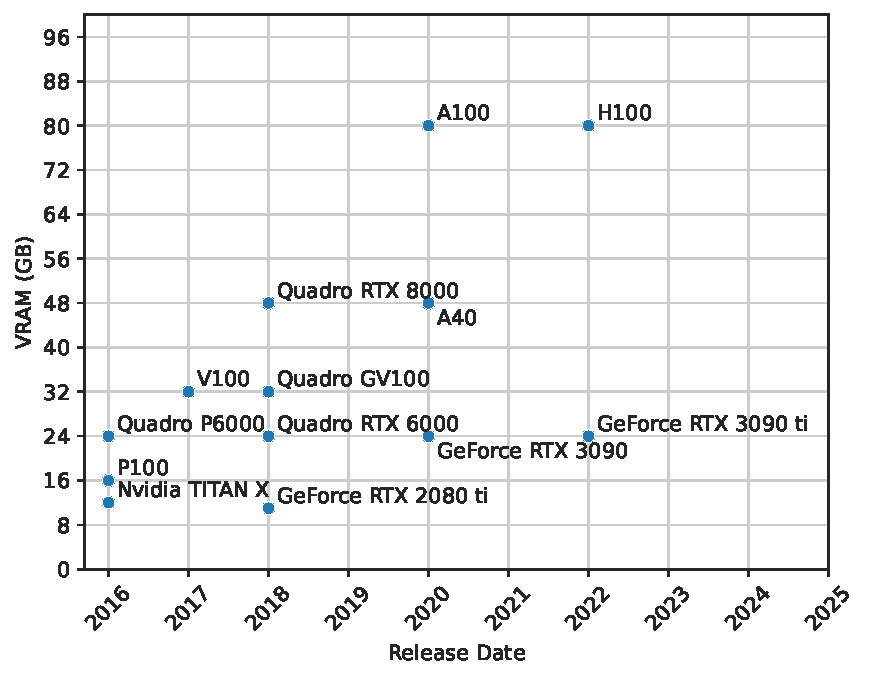
\includegraphics[width=\textwidth]{./figures/gpu-vram-over-time.pdf}
\end{figure}

Currently, the single GPU with the highest available memory produced by NVIDIA has 80GB available, which is almost double the amount of memory available to its direct predecessor 

A simple calculation shows that it would take roughly $530 \times 4 = 2120\texttt{GB}$ to simply hold the Megatron-Turing-NLG 530B \cite{smith2022megatronturingnlg} (the full model with 530 billion parameters) neural network model, which was released in 2022.
This is 350 times the amount of memory required by GPT-2, only requiring $1.5 \times 4 = 6\texttt{GB}$.

\begin{figure}[h]
    \caption{Model size over the past 4 years: ELMo \cite{peters2018elmo}, BERT \cite{devlin2018bert}, GPT-2 \cite{radford2019language}, Megatron-LM \cite{shoeybi2019megatronlm}, T-5 \cite{raffael2019t5}, Turing-NLG \cite{microsoft2020turingnlg}, GPT-3 \cite{brown2020gpt3}, Megatron-Turing-NLG \cite{smith2022megatronturingnlg}}
    \label{fig:model-size-over-time}
    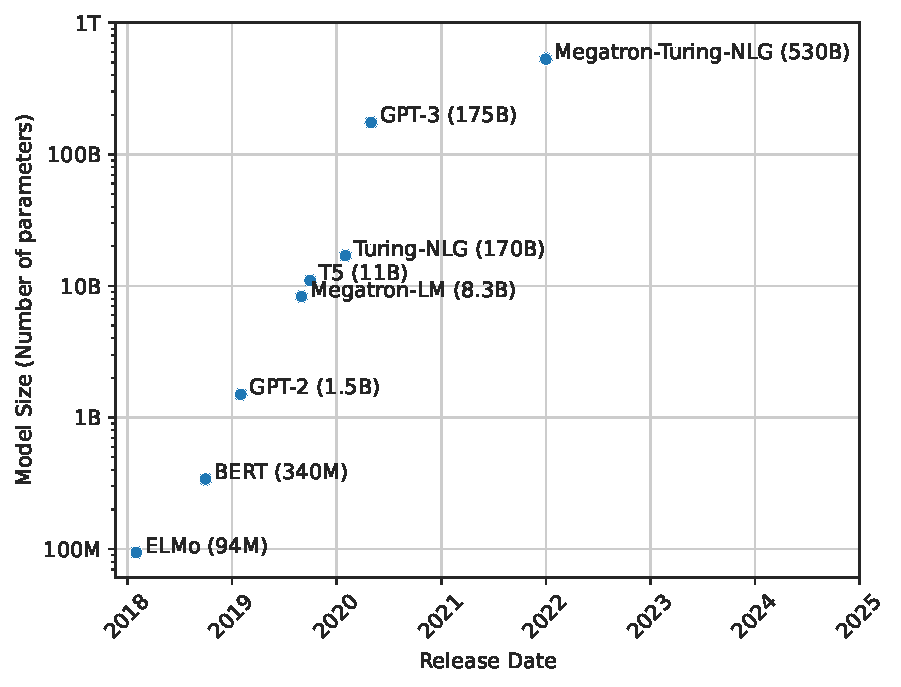
\includegraphics[width=\textwidth]{./figures/model-size-over-time.pdf}
\end{figure}


By comparison, the latest GPU released by NVIDIA earlier this year coded H100, has 80GB of HMB3 (high-bandwidth memory), only double the amount of RAM of its predecessor A100, released two years ago (see \autoref{fig:gpu-vram-over-time}).
It is therefore incredibly challenging to train today's state-of-the-art models with the current available hardware.

To tackle this problem, neural network practitioners have been studying and developing distributed computing techniques to train models that do not fit entirely in a single GPU's memory.
An early notable example of these techniques is AlexNet \cite{alexnet2012}. The architecture in \autoref{fig:alexnet} illustrates the basic idea that \cite{alexnet2012} introduces, which is to distribute the training of a single model across two GPUs.

\begin{figure}[h]
    \caption{AlexNet \cite{alexnet2012} architecture shows one of the first examples of model parallelism. The training of convolutional layers is split across two GPUs, as the size of the model during training exceeded the available memory of a single GPU.}
    \label{fig:alexnet}
    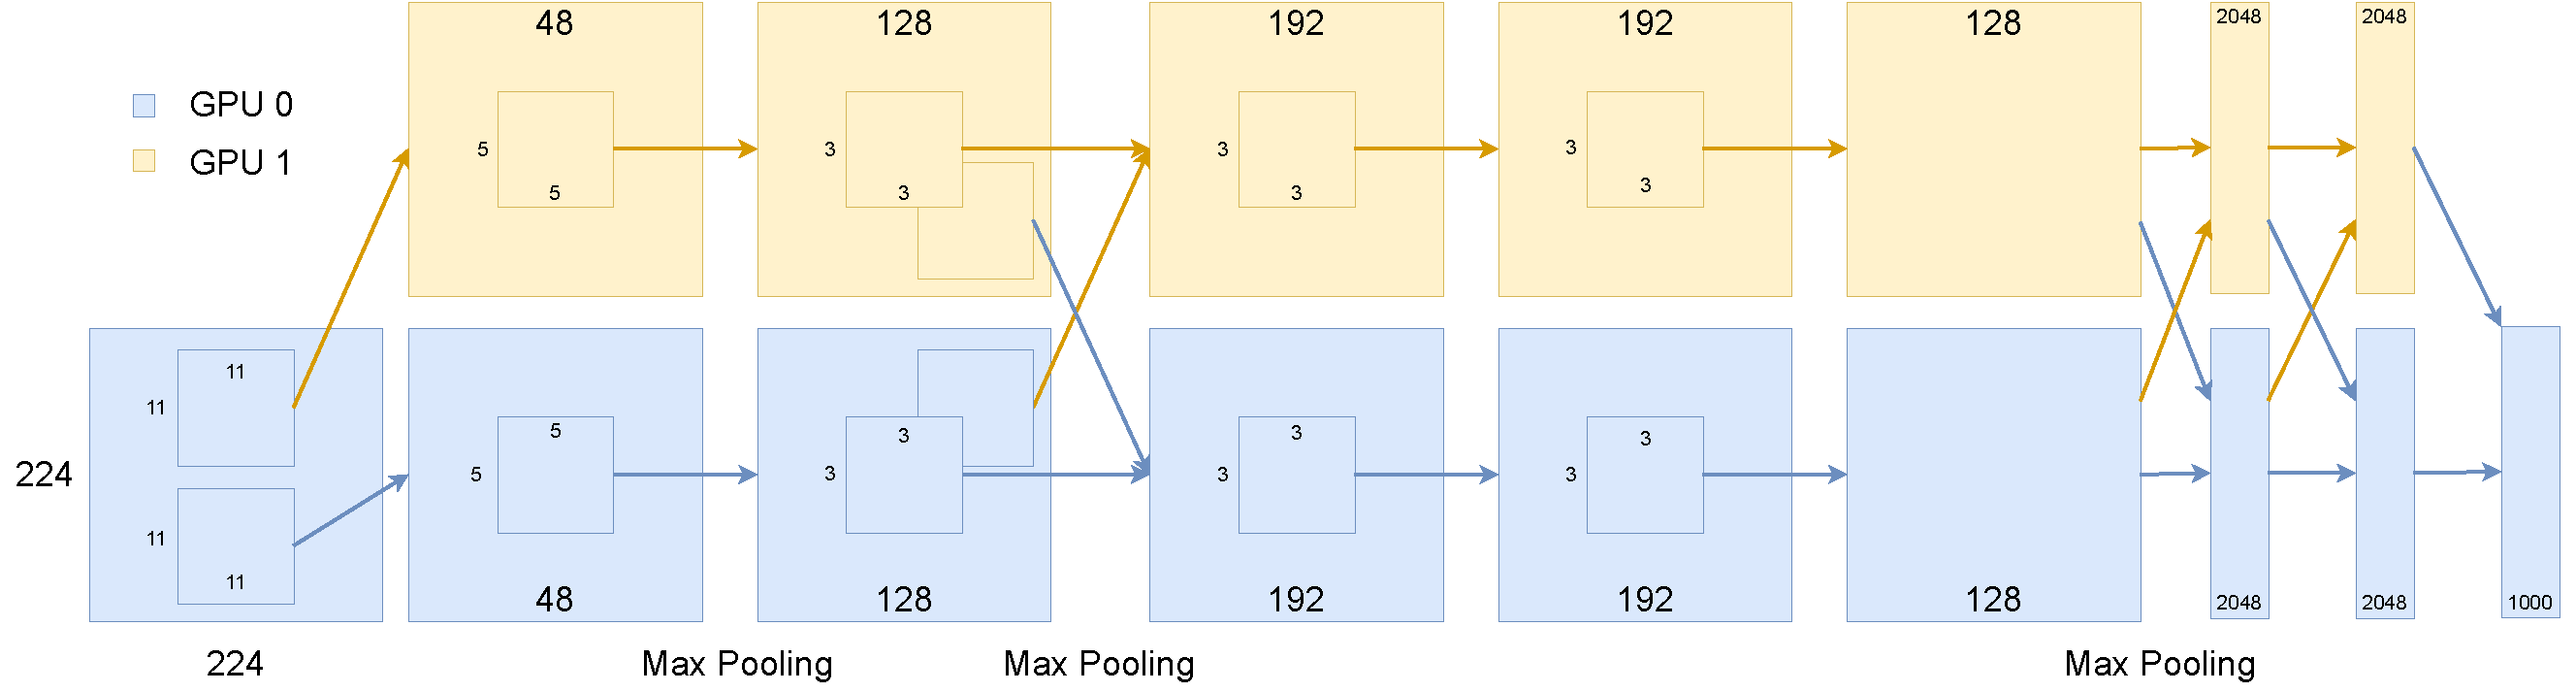
\includegraphics[width=\textwidth]{./figures/alexnet.pdf}
\end{figure}
